\subsection{Kết quả tái chạy mẫu tại máy biên tập}
Ngoài các bảng nhóm được giữ nguyên nguồn, một lần chạy mới được thực hiện trên ba ảnh
\texttt{bsds\_01}, \texttt{drive\_01}, \texttt{blob\_01}, bốn mức tỷ lệ từ config
và sáu toán tử $L,L_x,L_y,L_{xx},L_{xy},L_{yy}$. Nhân NumPy được lấy nguyên từ
repo tại commit \texttt{58e28e7}; đầu ra tham chiếu được tính thực sự bằng
ImageScience API với các thư viện của Fiji. Mỗi nhánh xuất 72 TIFF float32 không nén.

ImageJ dùng trong lần chạy là 1.54p, ImageScience là 3.1.0; Java là Temurin
21.0.12.1. FeatureJ được cài bằng bản build cục bộ từ nguồn chính thức
(\texttt{2.0.1-SNAPSHOT-local}). Lần xuất TIFF này gọi API ImageScience trực tiếp,
không đi qua hộp thoại plugin và không tạo ảnh chụp GUI. Vì khác nguồn và phiên bản
so với snapshot nhóm, các kết quả mới được báo cáo trong bảng riêng.

Python chạy ở phiên bản 3.12.10, NumPy 2.5.4
và tifffile 2026.10.15. Các tham số $\sigma$, bán kính kernel và
kiểu biên đọc từ config.yaml; bản đồ thô được so khớp sau khi loại dải biên.
Không dùng các PNG minh họa để tính sai số.

Có đủ 72 cặp hợp lệ, 18 cặp đạt STRICT và 54 cặp đạt RELAXED. Pearson nhỏ nhất là $0.99997591$, trung bình $0.99999803$; sai số cực đại tương đối lớn nhất là $0.8616\%$.

\begin{table*}[t]
\centering
\caption{Đối chiếu 72 bản đồ tính mới qua ImageScience API và nhân NumPy; relative error theo công thức~\eqref{eq:relmax}}
\begin{tabular}{lrrrrrr}
\toprule
Toán tử & $N$ & STRICT & RELAXED & Rel TB & Rel lớn nhất & Pearson nhỏ nhất\\
\midrule
Gauss & 12 & 12 & 0 & 7.105e-08 & 8.917e-08 & 1.00000000 \\
$L_x$ & 12 & 3 & 9 & 5.006e-04 & 8.866e-04 & 1.00000000 \\
$L_y$ & 12 & 3 & 9 & 5.006e-04 & 8.866e-04 & 1.00000000 \\
$L_{xx}$ & 12 & 0 & 12 & 4.070e-03 & 8.616e-03 & 0.99998026 \\
$L_{xy}$ & 12 & 0 & 12 & 1.002e-03 & 1.774e-03 & 1.00000000 \\
$L_{yy}$ & 12 & 0 & 12 & 4.202e-03 & 8.416e-03 & 0.99997591 \\
\bottomrule
\end{tabular}
\label{tab:local_sample}
\end{table*}

Các con số cho thấy phép đối chiếu mới tái hiện mức tương đồng cao trên tập mẫu:
Gaussian và một số đạo hàm bậc nhất đạt tiêu chí nghiêm ngặt, còn các bản đồ khác
có sai số hệ thống nằm dưới ngưỡng nới lỏng. Kết luận giới hạn trong 72 cặp đã đo;
không suy ra lại F1/IoU trên 25 ảnh từ lần chạy này. Thời gian trong log API là
thời gian của phép lọc đơn lẻ, chưa có quy trình lặp và loại warm-up, nên chưa
được dùng để công bố một hệ số tăng tốc Python--Fiji.

Các hình sau dùng chung thang màu cho cặp Python và ImageScience của từng toán tử.
Hàng sai khác có thanh màu riêng để nhìn vị trí sai số; độ đậm của hàng này phải
đọc cùng trị số trên colorbar. Hình hiển thị toàn ảnh, trong khi CSV tính điểm sau crop.
\begin{figure*}[tp]
\centering
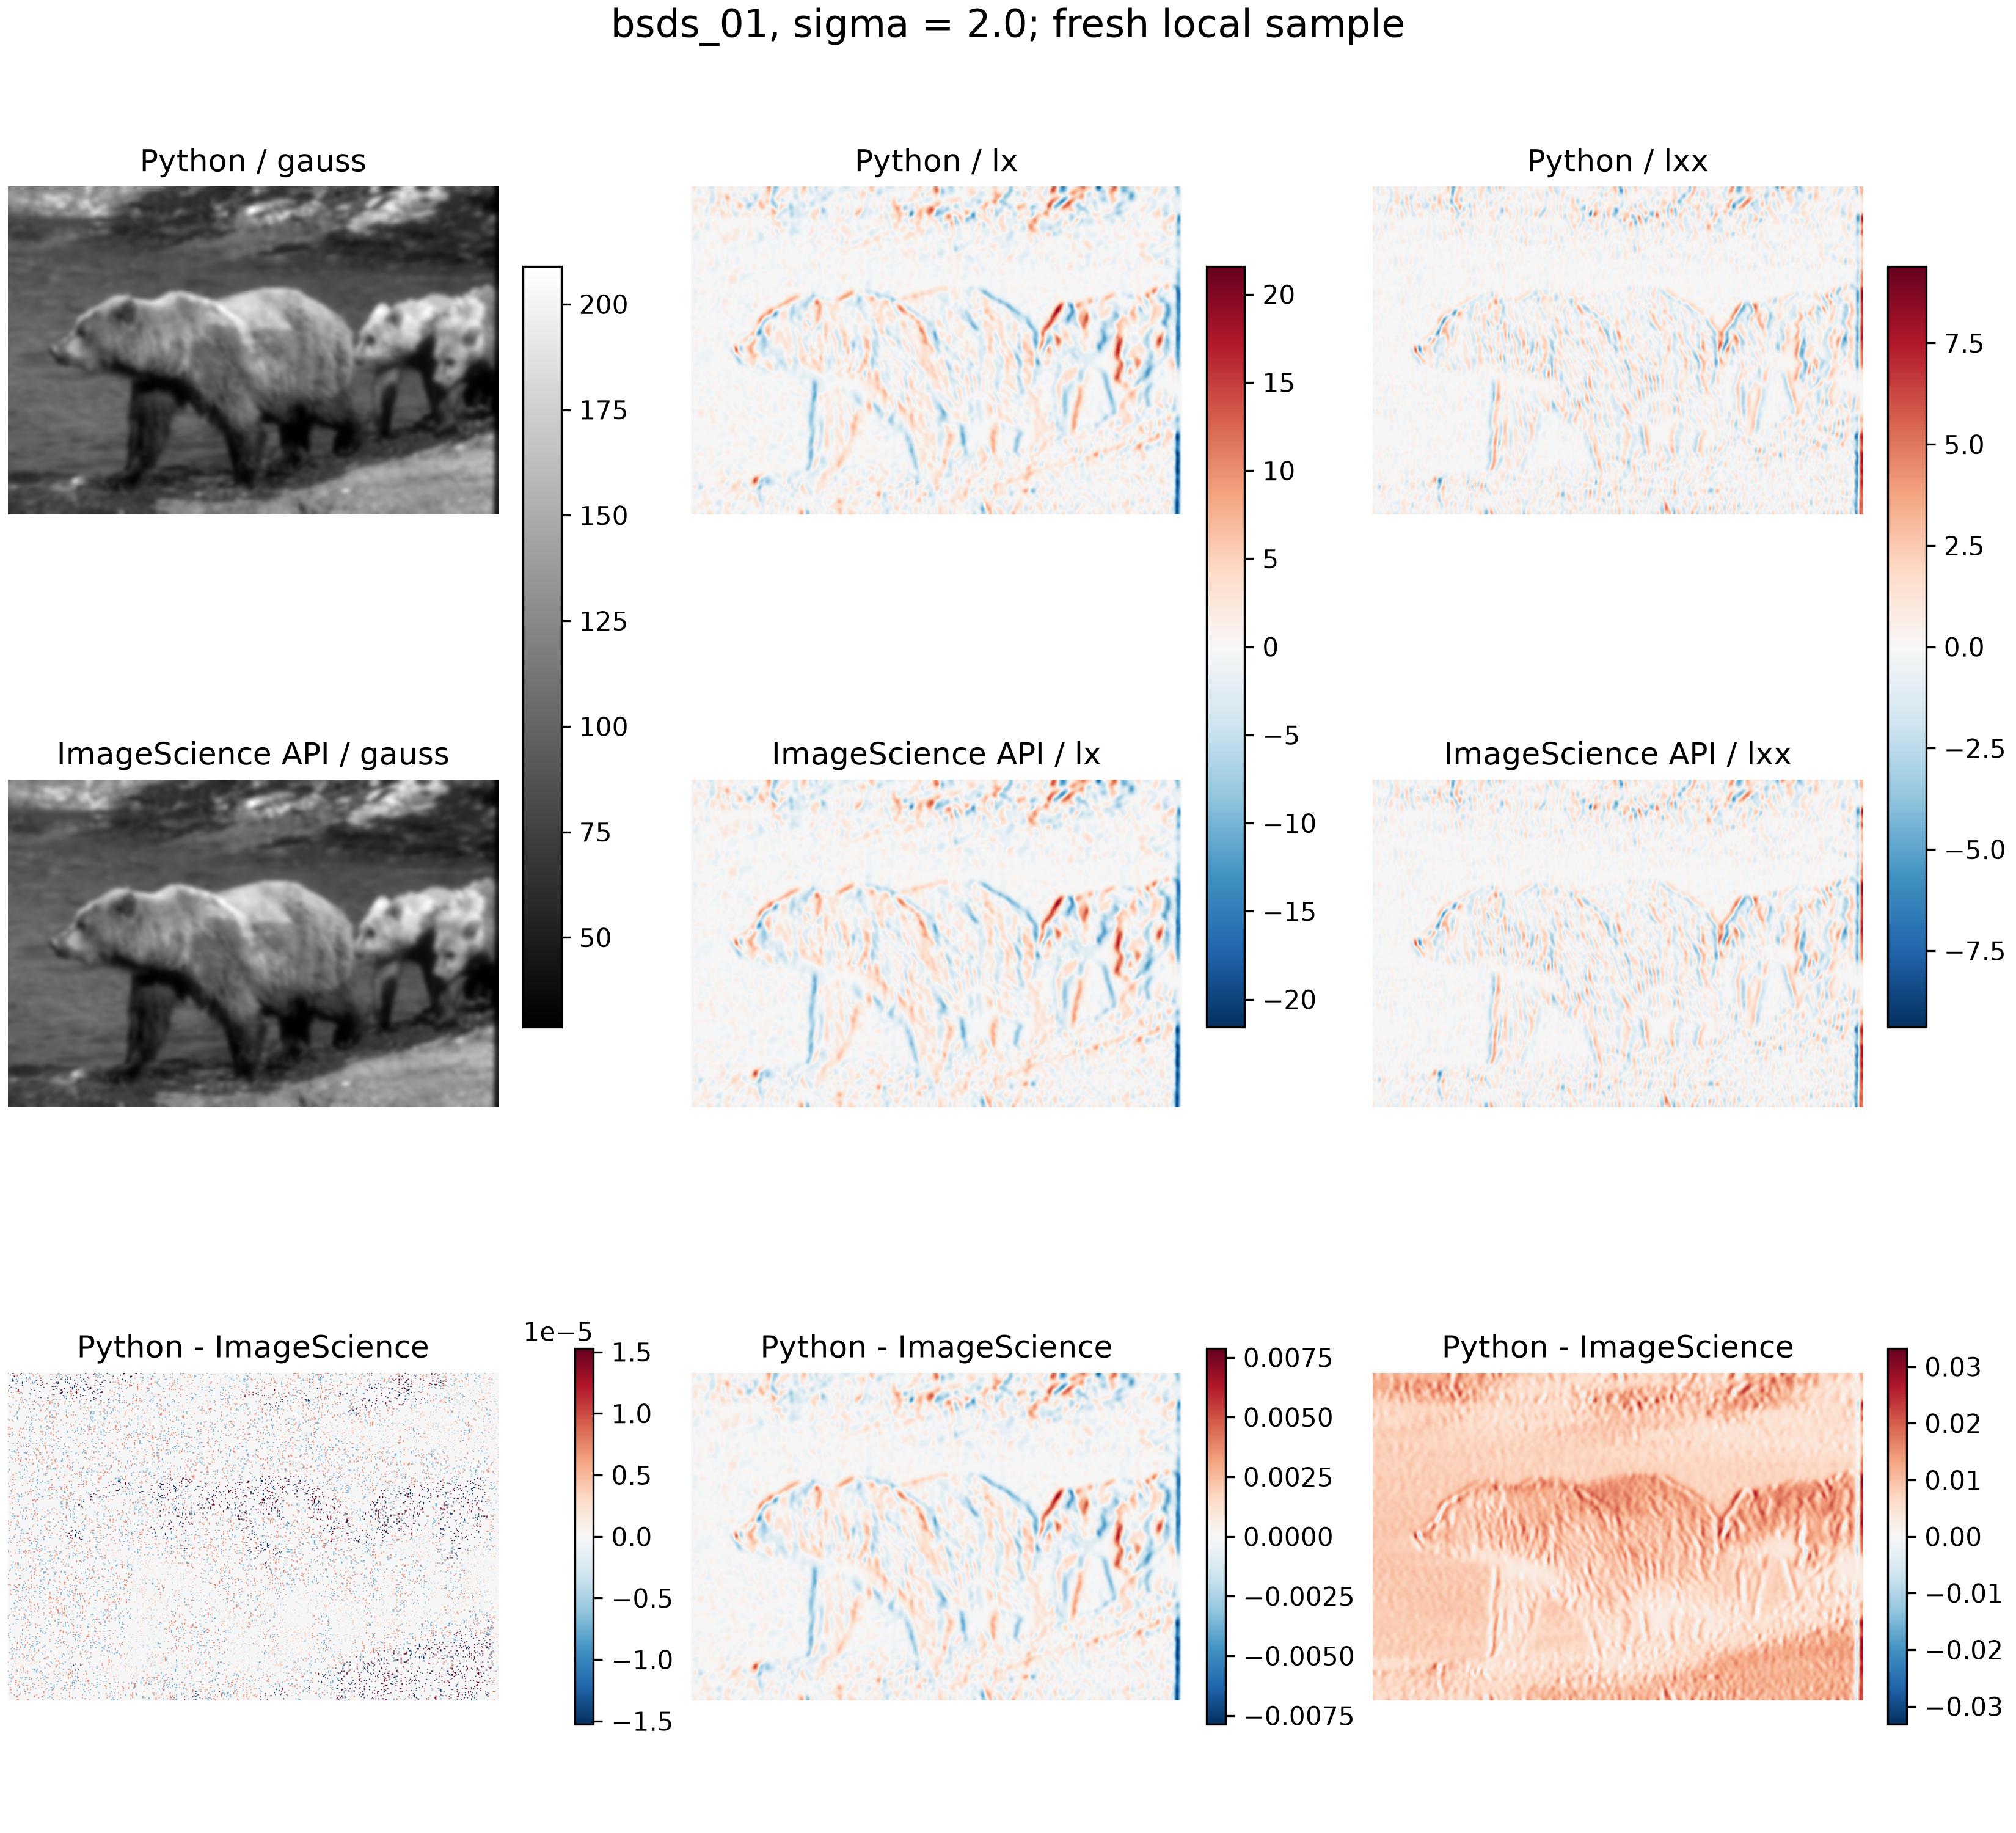
\includegraphics[width=0.82\textwidth]{figures/local_bsds_01_comparison.png}
\caption{Đối chiếu mẫu bsds\_01 tại $\sigma=2$: cột Gaussian, $L_x$, $L_{xx}$; hàng Python, ImageScience API và sai khác. Đây là dữ liệu tính mới, không phải ảnh chụp giao diện Fiji.}
\label{fig:local_bsds_01}
\end{figure*}

\begin{figure*}[tp]
\centering
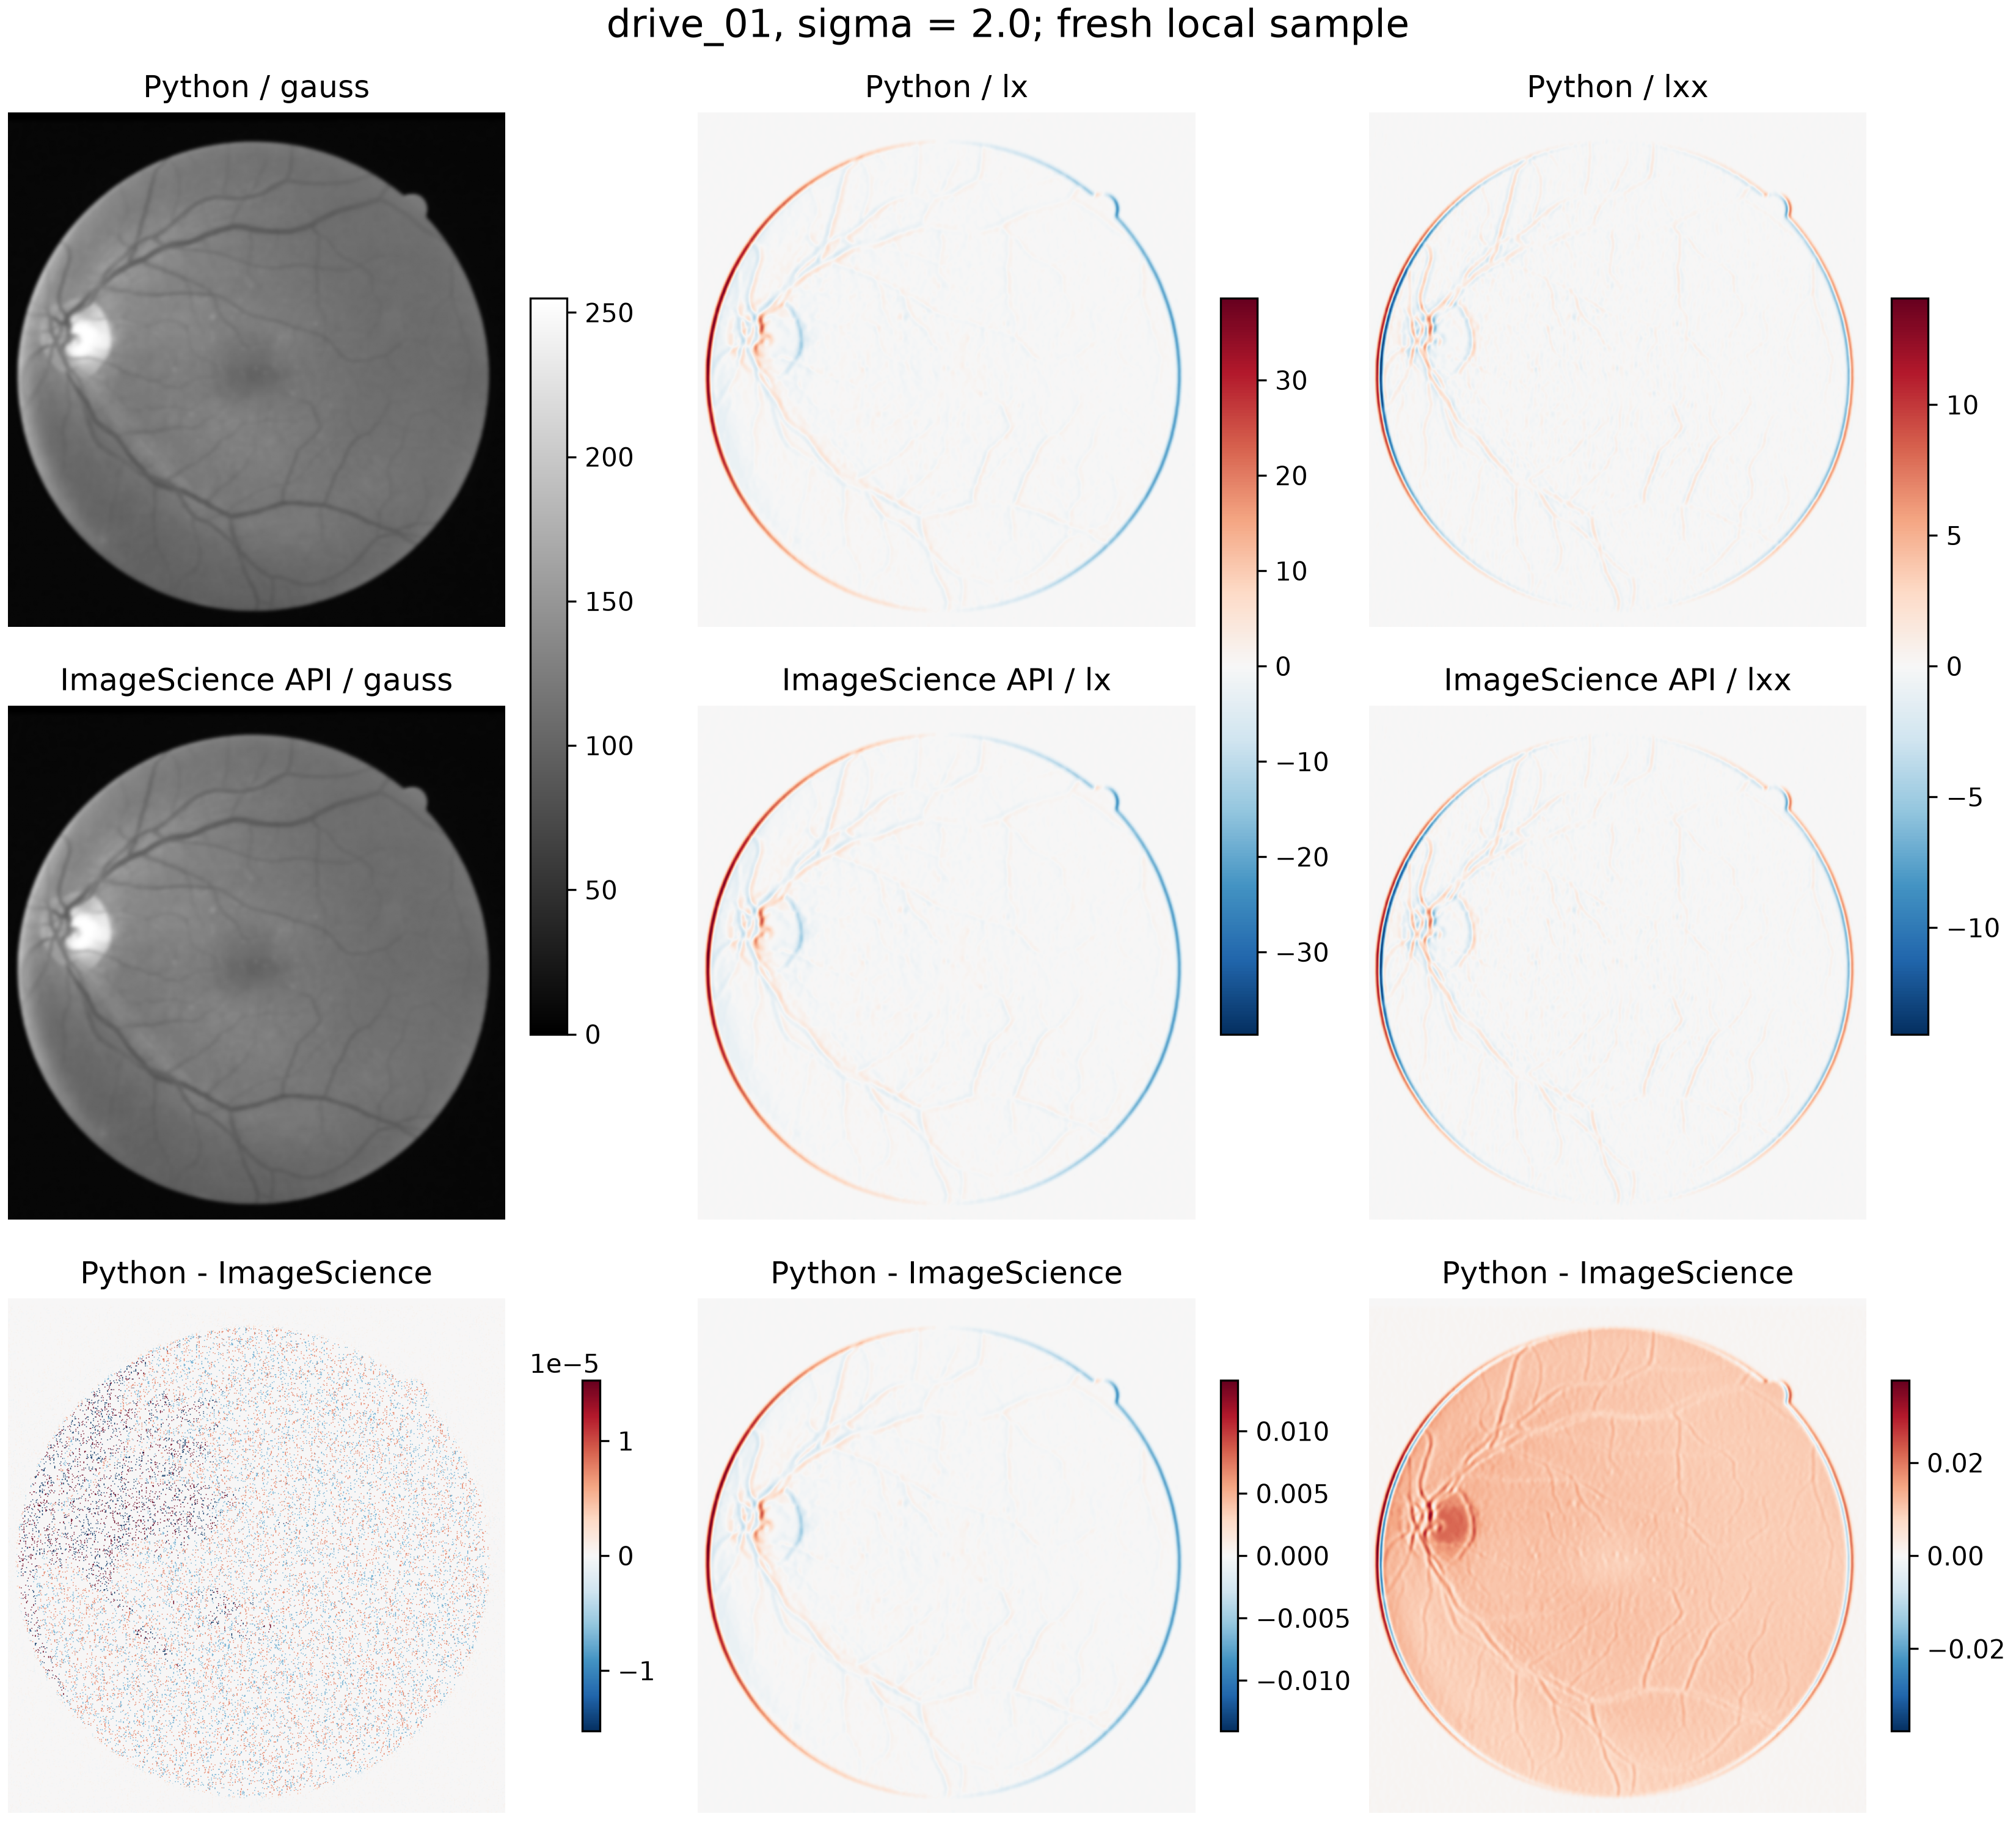
\includegraphics[width=0.82\textwidth]{figures/local_drive_01_comparison.png}
\caption{Đối chiếu mẫu drive\_01 tại $\sigma=2$: cột Gaussian, $L_x$, $L_{xx}$; hàng Python, ImageScience API và sai khác. Đây là dữ liệu tính mới, không phải ảnh chụp giao diện Fiji.}
\label{fig:local_drive_01}
\end{figure*}

\begin{figure*}[tp]
\centering
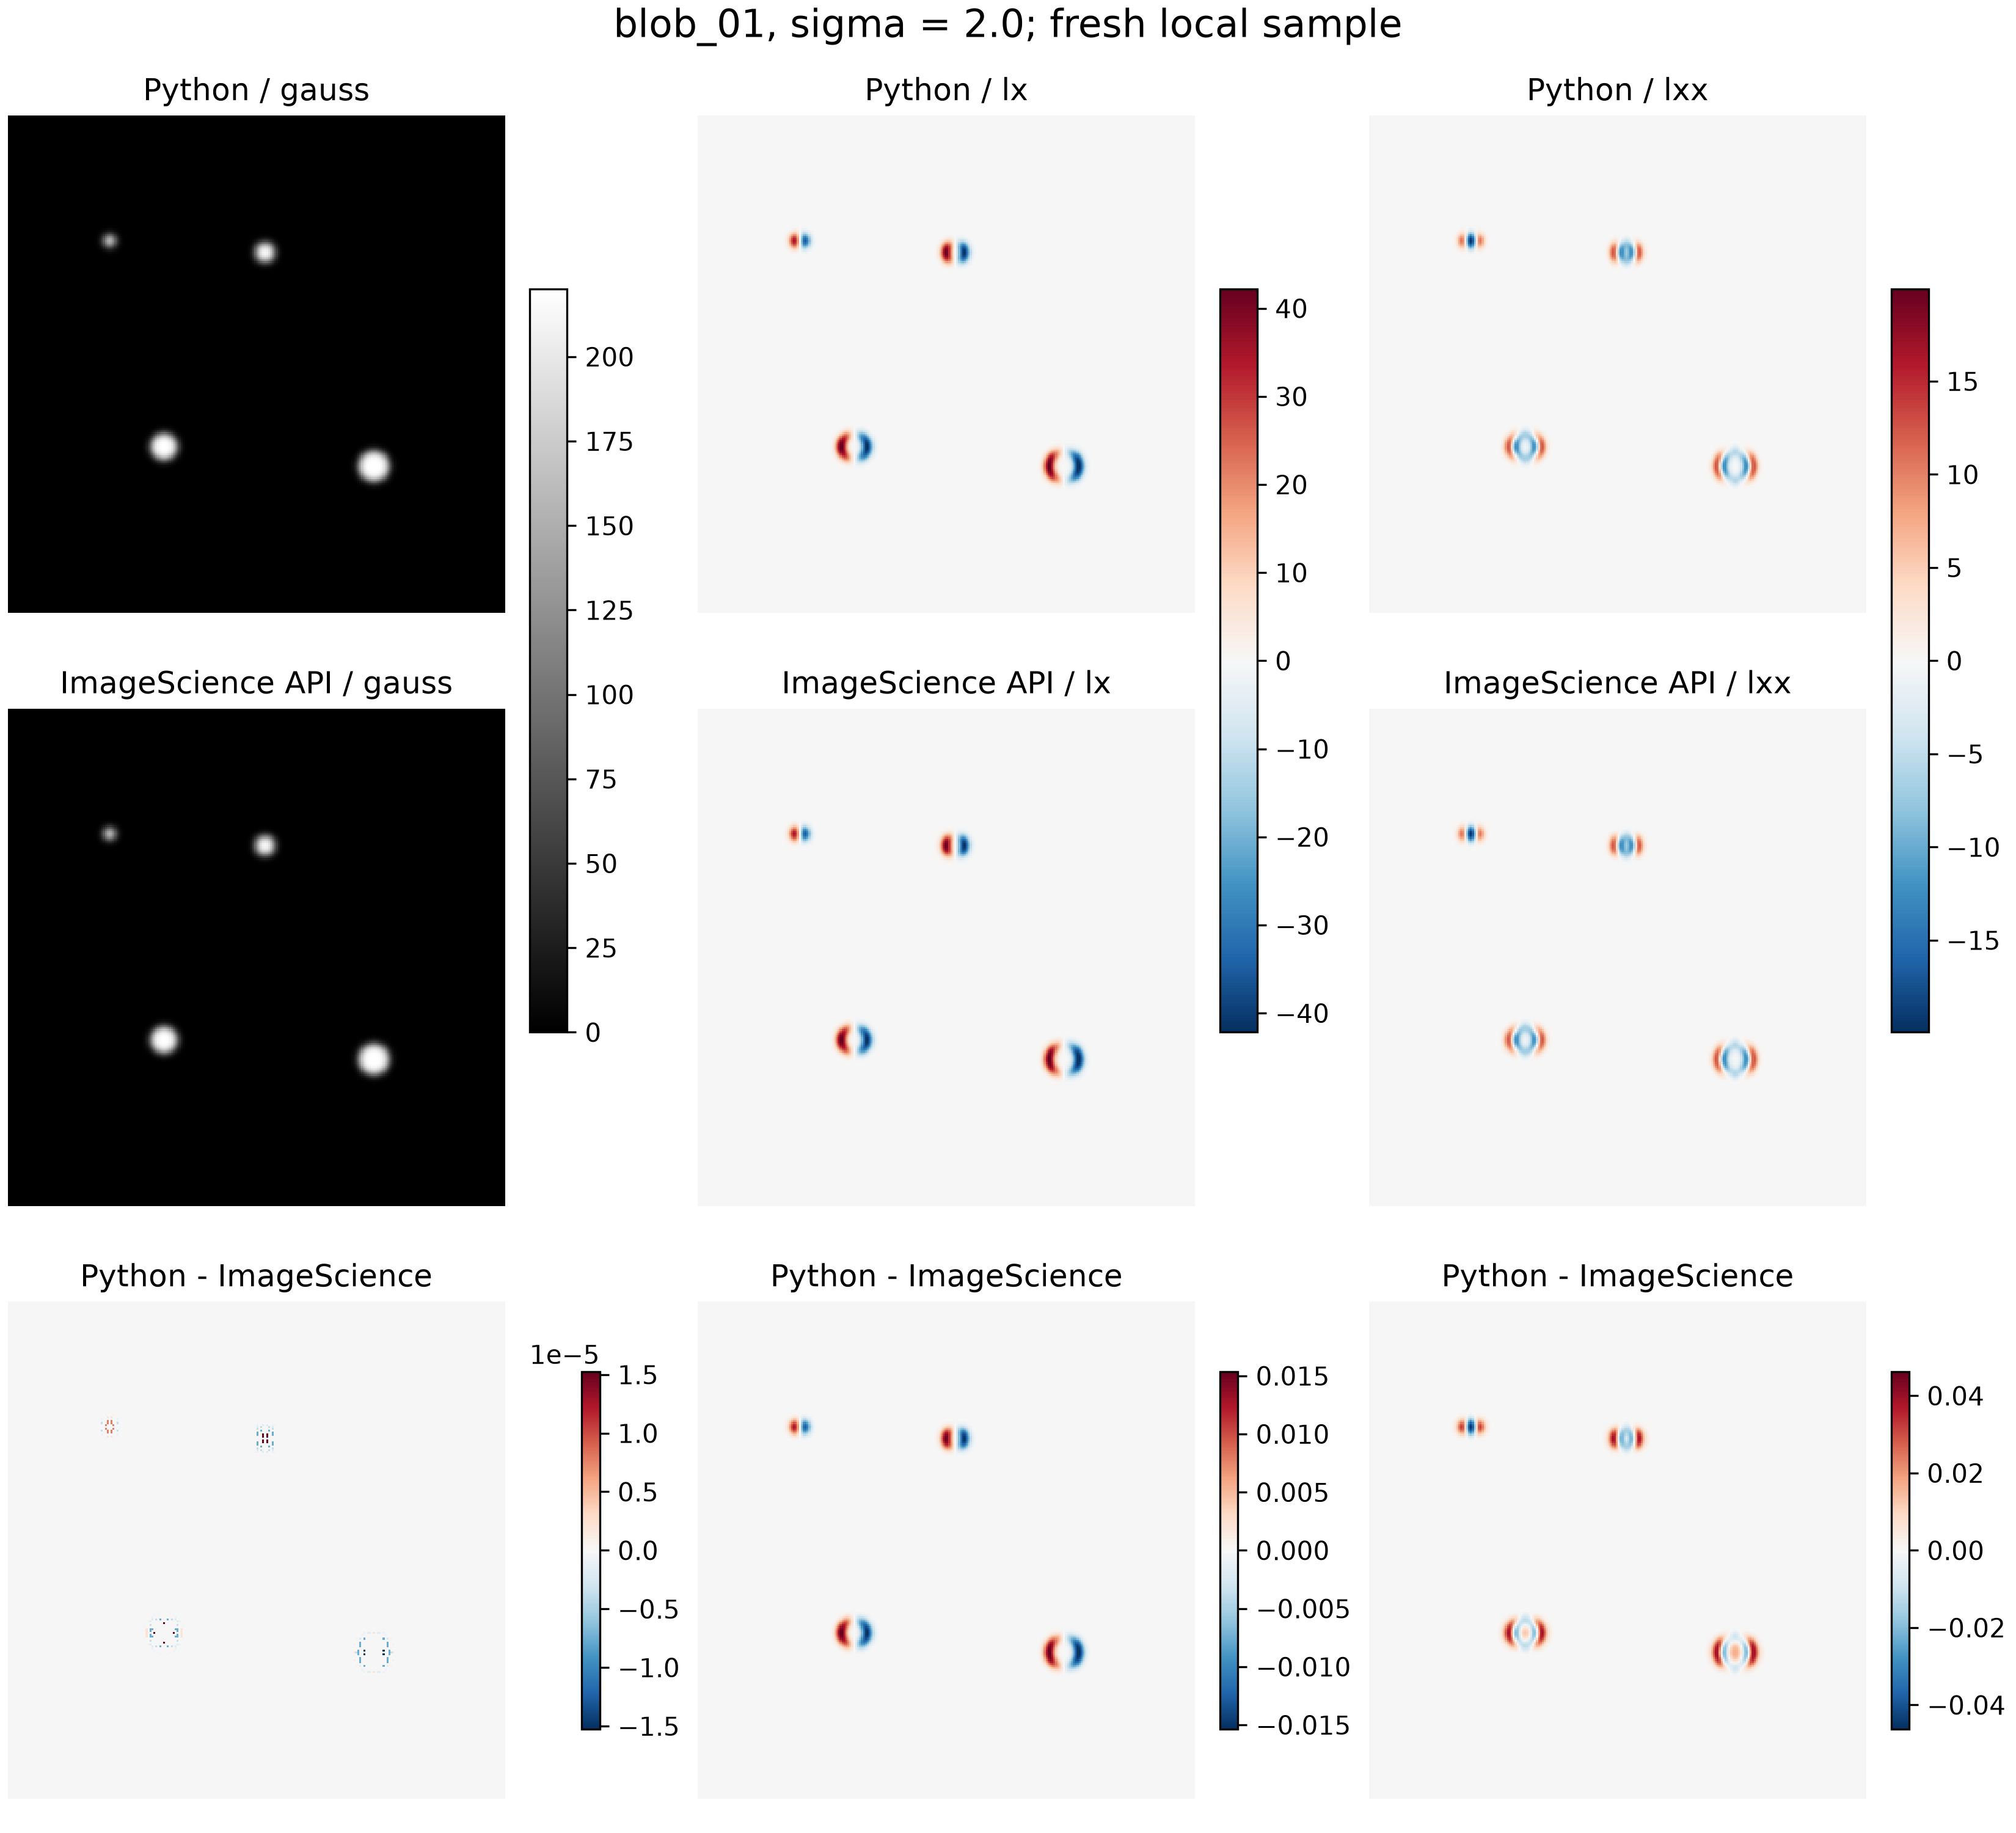
\includegraphics[width=0.82\textwidth]{figures/local_blob_01_comparison.png}
\caption{Đối chiếu mẫu blob\_01 tại $\sigma=2$: cột Gaussian, $L_x$, $L_{xx}$; hàng Python, ImageScience API và sai khác. Đây là dữ liệu tính mới, không phải ảnh chụp giao diện Fiji.}
\label{fig:local_blob_01}
\end{figure*}

